\documentclass[twoside]{book}

% Packages required by doxygen
\usepackage{fixltx2e}
\usepackage{calc}
\usepackage{doxygen}
\usepackage{graphicx}
\usepackage[utf8]{inputenc}
\usepackage{makeidx}
\usepackage{multicol}
\usepackage{multirow}
\PassOptionsToPackage{warn}{textcomp}
\usepackage{textcomp}
\usepackage[nointegrals]{wasysym}
\usepackage[table]{xcolor}

% Font selection
\usepackage[T1]{fontenc}
\usepackage{mathptmx}
\usepackage[scaled=.90]{helvet}
\usepackage{courier}
\usepackage{amssymb}
\usepackage{sectsty}
\renewcommand{\familydefault}{\sfdefault}
\allsectionsfont{%
  \fontseries{bc}\selectfont%
  \color{darkgray}%
}
\renewcommand{\DoxyLabelFont}{%
  \fontseries{bc}\selectfont%
  \color{darkgray}%
}
\newcommand{\+}{\discretionary{\mbox{\scriptsize$\hookleftarrow$}}{}{}}

% Page & text layout
\usepackage{geometry}
\geometry{%
  a4paper,%
  top=2.5cm,%
  bottom=2.5cm,%
  left=2.5cm,%
  right=2.5cm%
}
\tolerance=750
\hfuzz=15pt
\hbadness=750
\setlength{\emergencystretch}{15pt}
\setlength{\parindent}{0cm}
\setlength{\parskip}{0.2cm}
\makeatletter
\renewcommand{\paragraph}{%
  \@startsection{paragraph}{4}{0ex}{-1.0ex}{1.0ex}{%
    \normalfont\normalsize\bfseries\SS@parafont%
  }%
}
\renewcommand{\subparagraph}{%
  \@startsection{subparagraph}{5}{0ex}{-1.0ex}{1.0ex}{%
    \normalfont\normalsize\bfseries\SS@subparafont%
  }%
}
\makeatother

% Headers & footers
\usepackage{fancyhdr}
\pagestyle{fancyplain}
\fancyhead[LE]{\fancyplain{}{\bfseries\thepage}}
\fancyhead[CE]{\fancyplain{}{}}
\fancyhead[RE]{\fancyplain{}{\bfseries\leftmark}}
\fancyhead[LO]{\fancyplain{}{\bfseries\rightmark}}
\fancyhead[CO]{\fancyplain{}{}}
\fancyhead[RO]{\fancyplain{}{\bfseries\thepage}}
\fancyfoot[LE]{\fancyplain{}{}}
\fancyfoot[CE]{\fancyplain{}{}}
\fancyfoot[RE]{\fancyplain{}{\bfseries\scriptsize Generated on Mon Jul 10 2017 19\+:02\+:59 for My Project by Doxygen }}
\fancyfoot[LO]{\fancyplain{}{\bfseries\scriptsize Generated on Mon Jul 10 2017 19\+:02\+:59 for My Project by Doxygen }}
\fancyfoot[CO]{\fancyplain{}{}}
\fancyfoot[RO]{\fancyplain{}{}}
\renewcommand{\footrulewidth}{0.4pt}
\renewcommand{\chaptermark}[1]{%
  \markboth{#1}{}%
}
\renewcommand{\sectionmark}[1]{%
  \markright{\thesection\ #1}%
}

% Indices & bibliography
\usepackage{natbib}
\usepackage[titles]{tocloft}
\setcounter{tocdepth}{3}
\setcounter{secnumdepth}{5}
\makeindex

% Hyperlinks (required, but should be loaded last)
\usepackage{ifpdf}
\ifpdf
  \usepackage[pdftex,pagebackref=true]{hyperref}
\else
  \usepackage[ps2pdf,pagebackref=true]{hyperref}
\fi
\hypersetup{%
  colorlinks=true,%
  linkcolor=blue,%
  citecolor=blue,%
  unicode%
}

% Custom commands
\newcommand{\clearemptydoublepage}{%
  \newpage{\pagestyle{empty}\cleardoublepage}%
}


%===== C O N T E N T S =====

\begin{document}

% Titlepage & ToC
\hypersetup{pageanchor=false,
             bookmarks=true,
             bookmarksnumbered=true,
             pdfencoding=unicode
            }
\pagenumbering{roman}
\begin{titlepage}
\vspace*{7cm}
\begin{center}%
{\Large My Project }\\
\vspace*{1cm}
{\large Generated by Doxygen 1.8.8}\\
\vspace*{0.5cm}
{\small Mon Jul 10 2017 19:02:59}\\
\end{center}
\end{titlepage}
\clearemptydoublepage
\tableofcontents
\clearemptydoublepage
\pagenumbering{arabic}
\hypersetup{pageanchor=true}

%--- Begin generated contents ---
\chapter{File Index}
\section{File List}
Here is a list of all files with brief descriptions\+:\begin{DoxyCompactList}
\item\contentsline{section}{\hyperlink{config_8c}{config.\+c} }{\pageref{config_8c}}{}
\item\contentsline{section}{\hyperlink{config_8h}{config.\+h} }{\pageref{config_8h}}{}
\item\contentsline{section}{\hyperlink{core_8c}{core.\+c} }{\pageref{core_8c}}{}
\item\contentsline{section}{\hyperlink{core_8h}{core.\+h} }{\pageref{core_8h}}{}
\item\contentsline{section}{\hyperlink{wave_8c}{wave.\+c} }{\pageref{wave_8c}}{}
\end{DoxyCompactList}

\chapter{File Documentation}
\hypertarget{config_8c}{\section{config.\+c File Reference}
\label{config_8c}\index{config.\+c@{config.\+c}}
}
{\ttfamily \#include \char`\"{}config.\+h\char`\"{}}\\*
Include dependency graph for config.\+c\+:
\nopagebreak
\begin{figure}[H]
\begin{center}
\leavevmode
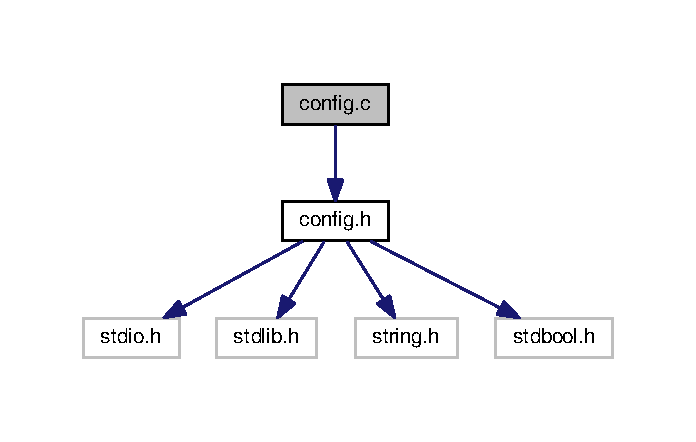
\includegraphics[width=334pt]{config_8c__incl}
\end{center}
\end{figure}
\subsection*{Macros}
\begin{DoxyCompactItemize}
\item 
\#define \hyperlink{config_8c_a3e937c42922f7601edb17b747602c471}{M\+A\+X\+L\+I\+N\+E}~100
\end{DoxyCompactItemize}
\subsection*{Functions}
\begin{DoxyCompactItemize}
\item 
double \hyperlink{config_8c_ad6a27e3b844adae13dbf6b465823a21e}{get\+C} ()
\item 
unsigned int \hyperlink{config_8c_a67c57ddf78540d69a30c741b356e7542}{get\+Data\+Size} ()
\item 
double \hyperlink{config_8c_aebdfcddd76cca4f1223533964ee4aa99}{get\+Shift} ()
\item 
unsigned int \hyperlink{config_8c_a9d725f3bbbc35aaf72f2631cc8fc624f}{get\+Simulation\+Steps} ()
\item 
bool \hyperlink{config_8c_aa29143a63f65543a6056d46a96e3084f}{is\+Gui} ()
\item 
int \hyperlink{config_8c_ade1b280acb4bd6500e99379c58263ed3}{read\+Config} (int argc, char $\ast$argv\mbox{[}$\,$\mbox{]})
\end{DoxyCompactItemize}
\subsection*{Variables}
\begin{DoxyCompactItemize}
\item 
double \hyperlink{config_8c_a2c09e929a6ea340fc9653cca414b11d3}{c}
\item 
double \hyperlink{config_8c_a96059d6a5d7c39fab3ae98297844903c}{shift}
\item 
unsigned int \hyperlink{config_8c_a843746ea29cdf8c55725f192780ff3d8}{array\+Size}
\item 
unsigned int \hyperlink{config_8c_aa03b8b6be1a1fb18504b20ae58b70643}{simulation\+Steps}
\item 
bool \hyperlink{config_8c_a25c29b3841901ddaf6ee35f75e4833d1}{show\+Gui}
\end{DoxyCompactItemize}


\subsection{Macro Definition Documentation}
\hypertarget{config_8c_a3e937c42922f7601edb17b747602c471}{\index{config.\+c@{config.\+c}!M\+A\+X\+L\+I\+N\+E@{M\+A\+X\+L\+I\+N\+E}}
\index{M\+A\+X\+L\+I\+N\+E@{M\+A\+X\+L\+I\+N\+E}!config.\+c@{config.\+c}}
\subsubsection[{M\+A\+X\+L\+I\+N\+E}]{\setlength{\rightskip}{0pt plus 5cm}\#define M\+A\+X\+L\+I\+N\+E~100}}\label{config_8c_a3e937c42922f7601edb17b747602c471}


\subsection{Function Documentation}
\hypertarget{config_8c_ad6a27e3b844adae13dbf6b465823a21e}{\index{config.\+c@{config.\+c}!get\+C@{get\+C}}
\index{get\+C@{get\+C}!config.\+c@{config.\+c}}
\subsubsection[{get\+C}]{\setlength{\rightskip}{0pt plus 5cm}double get\+C (
\begin{DoxyParamCaption}
\item[{void}]{}
\end{DoxyParamCaption}
)}}\label{config_8c_ad6a27e3b844adae13dbf6b465823a21e}
Returns a value for the length of each time step in the wave equation.

\begin{DoxyReturn}{Returns}
C 
\end{DoxyReturn}
\hypertarget{config_8c_a67c57ddf78540d69a30c741b356e7542}{\index{config.\+c@{config.\+c}!get\+Data\+Size@{get\+Data\+Size}}
\index{get\+Data\+Size@{get\+Data\+Size}!config.\+c@{config.\+c}}
\subsubsection[{get\+Data\+Size}]{\setlength{\rightskip}{0pt plus 5cm}unsigned int get\+Data\+Size (
\begin{DoxyParamCaption}
\item[{void}]{}
\end{DoxyParamCaption}
)}}\label{config_8c_a67c57ddf78540d69a30c741b356e7542}
Returns array size which is the length of the wave.

\begin{DoxyReturn}{Returns}
array size 
\end{DoxyReturn}
\hypertarget{config_8c_aebdfcddd76cca4f1223533964ee4aa99}{\index{config.\+c@{config.\+c}!get\+Shift@{get\+Shift}}
\index{get\+Shift@{get\+Shift}!config.\+c@{config.\+c}}
\subsubsection[{get\+Shift}]{\setlength{\rightskip}{0pt plus 5cm}double get\+Shift (
\begin{DoxyParamCaption}
\item[{void}]{}
\end{DoxyParamCaption}
)}}\label{config_8c_aebdfcddd76cca4f1223533964ee4aa99}
Returns the shift value which is the difference of the inital waves.

\begin{DoxyReturn}{Returns}
shift 
\end{DoxyReturn}
\hypertarget{config_8c_a9d725f3bbbc35aaf72f2631cc8fc624f}{\index{config.\+c@{config.\+c}!get\+Simulation\+Steps@{get\+Simulation\+Steps}}
\index{get\+Simulation\+Steps@{get\+Simulation\+Steps}!config.\+c@{config.\+c}}
\subsubsection[{get\+Simulation\+Steps}]{\setlength{\rightskip}{0pt plus 5cm}unsigned int get\+Simulation\+Steps (
\begin{DoxyParamCaption}
\item[{void}]{}
\end{DoxyParamCaption}
)}}\label{config_8c_a9d725f3bbbc35aaf72f2631cc8fc624f}
Returns the Count of Steps which are executed before the program exits.

\begin{DoxyReturn}{Returns}
simulation steps 
\end{DoxyReturn}
\hypertarget{config_8c_aa29143a63f65543a6056d46a96e3084f}{\index{config.\+c@{config.\+c}!is\+Gui@{is\+Gui}}
\index{is\+Gui@{is\+Gui}!config.\+c@{config.\+c}}
\subsubsection[{is\+Gui}]{\setlength{\rightskip}{0pt plus 5cm}bool is\+Gui (
\begin{DoxyParamCaption}
\item[{void}]{}
\end{DoxyParamCaption}
)}}\label{config_8c_aa29143a63f65543a6056d46a96e3084f}
Returns whether the gui shall be shown or not.

\begin{DoxyReturn}{Returns}
1 = show; 0 = do not show 
\end{DoxyReturn}
\hypertarget{config_8c_ade1b280acb4bd6500e99379c58263ed3}{\index{config.\+c@{config.\+c}!read\+Config@{read\+Config}}
\index{read\+Config@{read\+Config}!config.\+c@{config.\+c}}
\subsubsection[{read\+Config}]{\setlength{\rightskip}{0pt plus 5cm}int read\+Config (
\begin{DoxyParamCaption}
\item[{int}]{argc, }
\item[{char $\ast$}]{argv\mbox{[}$\,$\mbox{]}}
\end{DoxyParamCaption}
)}}\label{config_8c_ade1b280acb4bd6500e99379c58263ed3}
Reads the given config and program arguments and provides those for other parts of the program.


\begin{DoxyParams}{Parameters}
{\em argc} & argument count of program \\
\hline
{\em argv} & arguments of program \\
\hline
\end{DoxyParams}


\subsection{Variable Documentation}
\hypertarget{config_8c_a843746ea29cdf8c55725f192780ff3d8}{\index{config.\+c@{config.\+c}!array\+Size@{array\+Size}}
\index{array\+Size@{array\+Size}!config.\+c@{config.\+c}}
\subsubsection[{array\+Size}]{\setlength{\rightskip}{0pt plus 5cm}unsigned int array\+Size}}\label{config_8c_a843746ea29cdf8c55725f192780ff3d8}
\hypertarget{config_8c_a2c09e929a6ea340fc9653cca414b11d3}{\index{config.\+c@{config.\+c}!c@{c}}
\index{c@{c}!config.\+c@{config.\+c}}
\subsubsection[{c}]{\setlength{\rightskip}{0pt plus 5cm}double c}}\label{config_8c_a2c09e929a6ea340fc9653cca414b11d3}
\hypertarget{config_8c_a96059d6a5d7c39fab3ae98297844903c}{\index{config.\+c@{config.\+c}!shift@{shift}}
\index{shift@{shift}!config.\+c@{config.\+c}}
\subsubsection[{shift}]{\setlength{\rightskip}{0pt plus 5cm}double shift}}\label{config_8c_a96059d6a5d7c39fab3ae98297844903c}
\hypertarget{config_8c_a25c29b3841901ddaf6ee35f75e4833d1}{\index{config.\+c@{config.\+c}!show\+Gui@{show\+Gui}}
\index{show\+Gui@{show\+Gui}!config.\+c@{config.\+c}}
\subsubsection[{show\+Gui}]{\setlength{\rightskip}{0pt plus 5cm}bool show\+Gui}}\label{config_8c_a25c29b3841901ddaf6ee35f75e4833d1}
\hypertarget{config_8c_aa03b8b6be1a1fb18504b20ae58b70643}{\index{config.\+c@{config.\+c}!simulation\+Steps@{simulation\+Steps}}
\index{simulation\+Steps@{simulation\+Steps}!config.\+c@{config.\+c}}
\subsubsection[{simulation\+Steps}]{\setlength{\rightskip}{0pt plus 5cm}unsigned int simulation\+Steps}}\label{config_8c_aa03b8b6be1a1fb18504b20ae58b70643}

\hypertarget{config_8h}{\section{config.\+h File Reference}
\label{config_8h}\index{config.\+h@{config.\+h}}
}
{\ttfamily \#include $<$stdio.\+h$>$}\\*
{\ttfamily \#include $<$stdlib.\+h$>$}\\*
{\ttfamily \#include $<$string.\+h$>$}\\*
{\ttfamily \#include $<$stdbool.\+h$>$}\\*
Include dependency graph for config.\+h\+:
\nopagebreak
\begin{figure}[H]
\begin{center}
\leavevmode
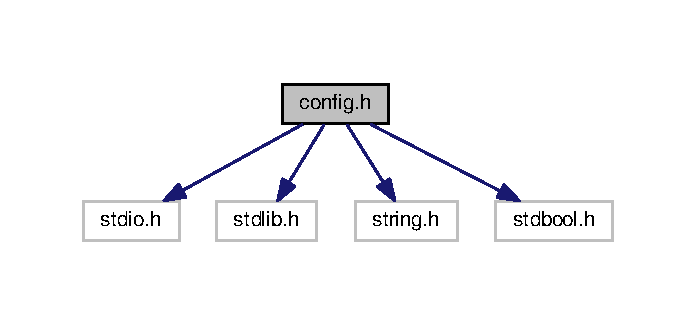
\includegraphics[width=334pt]{config_8h__incl}
\end{center}
\end{figure}
This graph shows which files directly or indirectly include this file\+:
\nopagebreak
\begin{figure}[H]
\begin{center}
\leavevmode
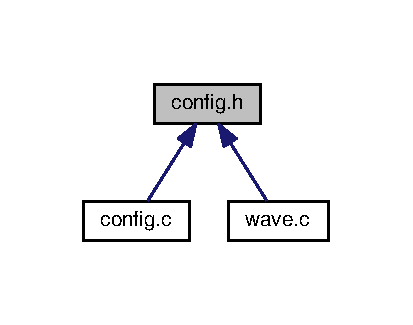
\includegraphics[width=198pt]{config_8h__dep__incl}
\end{center}
\end{figure}
\subsection*{Functions}
\begin{DoxyCompactItemize}
\item 
double \hyperlink{config_8h_ae1637d8a2455db5c94c995eeaed00974}{get\+C} (void)
\item 
unsigned int \hyperlink{config_8h_ae65dd4e7e60595bedf09ddb834260695}{get\+Data\+Size} (void)
\item 
double \hyperlink{config_8h_ac2b0b5d202520eb3b5b9a7536792a336}{get\+Shift} (void)
\item 
unsigned int \hyperlink{config_8h_adf961c4f62a2fb366d8ea1b97f7c1476}{get\+Simulation\+Steps} (void)
\item 
bool \hyperlink{config_8h_a87110e2d36b473e649ad7442e32a2114}{is\+Gui} (void)
\item 
int \hyperlink{config_8h_ade1b280acb4bd6500e99379c58263ed3}{read\+Config} (int argc, char $\ast$argv\mbox{[}$\,$\mbox{]})
\end{DoxyCompactItemize}


\subsection{Function Documentation}
\hypertarget{config_8h_ae1637d8a2455db5c94c995eeaed00974}{\index{config.\+h@{config.\+h}!get\+C@{get\+C}}
\index{get\+C@{get\+C}!config.\+h@{config.\+h}}
\subsubsection[{get\+C}]{\setlength{\rightskip}{0pt plus 5cm}double get\+C (
\begin{DoxyParamCaption}
\item[{void}]{}
\end{DoxyParamCaption}
)}}\label{config_8h_ae1637d8a2455db5c94c995eeaed00974}
Returns a value for the length of each time step in the wave equation.

\begin{DoxyReturn}{Returns}
C 
\end{DoxyReturn}
\hypertarget{config_8h_ae65dd4e7e60595bedf09ddb834260695}{\index{config.\+h@{config.\+h}!get\+Data\+Size@{get\+Data\+Size}}
\index{get\+Data\+Size@{get\+Data\+Size}!config.\+h@{config.\+h}}
\subsubsection[{get\+Data\+Size}]{\setlength{\rightskip}{0pt plus 5cm}unsigned int get\+Data\+Size (
\begin{DoxyParamCaption}
\item[{void}]{}
\end{DoxyParamCaption}
)}}\label{config_8h_ae65dd4e7e60595bedf09ddb834260695}
Returns array size which is the length of the wave.

\begin{DoxyReturn}{Returns}
array size 
\end{DoxyReturn}
\hypertarget{config_8h_ac2b0b5d202520eb3b5b9a7536792a336}{\index{config.\+h@{config.\+h}!get\+Shift@{get\+Shift}}
\index{get\+Shift@{get\+Shift}!config.\+h@{config.\+h}}
\subsubsection[{get\+Shift}]{\setlength{\rightskip}{0pt plus 5cm}double get\+Shift (
\begin{DoxyParamCaption}
\item[{void}]{}
\end{DoxyParamCaption}
)}}\label{config_8h_ac2b0b5d202520eb3b5b9a7536792a336}
Returns the shift value which is the difference of the inital waves.

\begin{DoxyReturn}{Returns}
shift 
\end{DoxyReturn}
\hypertarget{config_8h_adf961c4f62a2fb366d8ea1b97f7c1476}{\index{config.\+h@{config.\+h}!get\+Simulation\+Steps@{get\+Simulation\+Steps}}
\index{get\+Simulation\+Steps@{get\+Simulation\+Steps}!config.\+h@{config.\+h}}
\subsubsection[{get\+Simulation\+Steps}]{\setlength{\rightskip}{0pt plus 5cm}unsigned int get\+Simulation\+Steps (
\begin{DoxyParamCaption}
\item[{void}]{}
\end{DoxyParamCaption}
)}}\label{config_8h_adf961c4f62a2fb366d8ea1b97f7c1476}
Returns the Count of Steps which are executed before the program exits.

\begin{DoxyReturn}{Returns}
simulation steps 
\end{DoxyReturn}
\hypertarget{config_8h_a87110e2d36b473e649ad7442e32a2114}{\index{config.\+h@{config.\+h}!is\+Gui@{is\+Gui}}
\index{is\+Gui@{is\+Gui}!config.\+h@{config.\+h}}
\subsubsection[{is\+Gui}]{\setlength{\rightskip}{0pt plus 5cm}bool is\+Gui (
\begin{DoxyParamCaption}
\item[{void}]{}
\end{DoxyParamCaption}
)}}\label{config_8h_a87110e2d36b473e649ad7442e32a2114}
Returns whether the gui shall be shown or not.

\begin{DoxyReturn}{Returns}
1 = show; 0 = do not show 
\end{DoxyReturn}
\hypertarget{config_8h_ade1b280acb4bd6500e99379c58263ed3}{\index{config.\+h@{config.\+h}!read\+Config@{read\+Config}}
\index{read\+Config@{read\+Config}!config.\+h@{config.\+h}}
\subsubsection[{read\+Config}]{\setlength{\rightskip}{0pt plus 5cm}int read\+Config (
\begin{DoxyParamCaption}
\item[{int}]{argc, }
\item[{char $\ast$}]{argv\mbox{[}$\,$\mbox{]}}
\end{DoxyParamCaption}
)}}\label{config_8h_ade1b280acb4bd6500e99379c58263ed3}
Reads the given config and program arguments and provides those for other parts of the program.


\begin{DoxyParams}{Parameters}
{\em argc} & argument count of program \\
\hline
{\em argv} & arguments of program \\
\hline
\end{DoxyParams}

\hypertarget{core_8c}{\section{core.\+c File Reference}
\label{core_8c}\index{core.\+c@{core.\+c}}
}
{\ttfamily \#include \char`\"{}core.\+h\char`\"{}}\\*
Include dependency graph for core.\+c\+:
\nopagebreak
\begin{figure}[H]
\begin{center}
\leavevmode
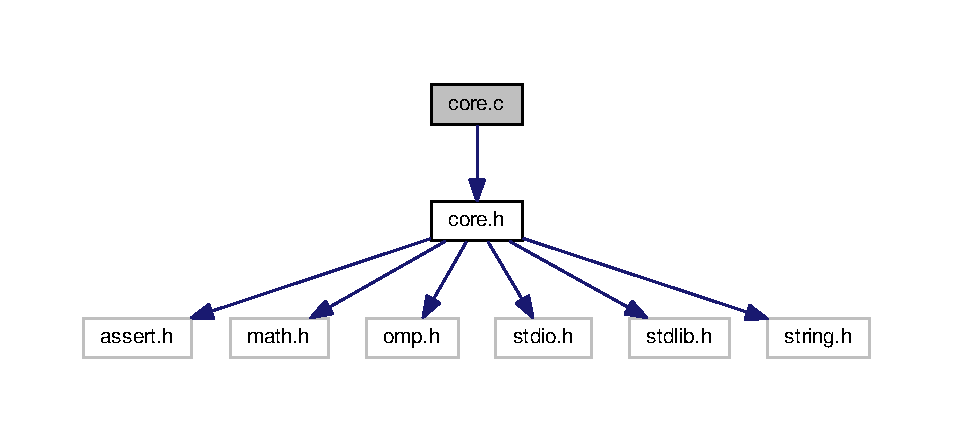
\includegraphics[width=350pt]{core_8c__incl}
\end{center}
\end{figure}
\subsection*{Functions}
\begin{DoxyCompactItemize}
\item 
void \hyperlink{core_8c_a2c792ddc06951a4c4d72722e4779f144}{init} (double c\+Factor, unsigned int t\+Points, double shift\+Factor)
\item 
void \hyperlink{core_8c_a1f451daf160cbacfab1e7b495789750e}{simulate} ()
\item 
void \hyperlink{core_8c_a7437b254e19e7e12fc2ec99945f4ecea}{output} ()
\item 
double $\ast$ \hyperlink{core_8c_a52f1b48db944eec28aa0e073d6696c6e}{get\+New\+Values} ()
\item 
int \hyperlink{core_8c_a1779d5453fa635501dab78cf8c15a878}{get\+Array\+Size} ()
\item 
void \hyperlink{core_8c_a74a45d2648335936561898c390281a6a}{terminate} ()
\end{DoxyCompactItemize}
\subsection*{Variables}
\begin{DoxyCompactItemize}
\item 
double $\ast$ \hyperlink{core_8c_a2098158062e3e63fce7d2575b324c386}{values}
\item 
double $\ast$ \hyperlink{core_8c_a4ff5e6005029031acf0e76184141b0b1}{oldval}
\item 
double $\ast$ \hyperlink{core_8c_af3a59edd41b5d1449b69355fdffd29a0}{newval}
\item 
int \hyperlink{core_8c_a050bf9eb9b046d41394b6169721a2fde}{arr\+Len}
\item 
int \hyperlink{core_8c_a1ea5d0cb93f22f7d0fdf804bd68c3326}{mode} = 0
\item 
double \hyperlink{core_8c_a2c09e929a6ea340fc9653cca414b11d3}{c} = 0.\+1
\item 
double \hyperlink{core_8c_a96059d6a5d7c39fab3ae98297844903c}{shift}
\end{DoxyCompactItemize}


\subsection{Detailed Description}
Implements the core of the algorithm. 

\subsection{Function Documentation}
\hypertarget{core_8c_a1779d5453fa635501dab78cf8c15a878}{\index{core.\+c@{core.\+c}!get\+Array\+Size@{get\+Array\+Size}}
\index{get\+Array\+Size@{get\+Array\+Size}!core.\+c@{core.\+c}}
\subsubsection[{get\+Array\+Size}]{\setlength{\rightskip}{0pt plus 5cm}int get\+Array\+Size (
\begin{DoxyParamCaption}
\item[{void}]{}
\end{DoxyParamCaption}
)}}\label{core_8c_a1779d5453fa635501dab78cf8c15a878}
Return lengths of the value arrays

\begin{DoxyReturn}{Returns}
lengths 
\end{DoxyReturn}
\hypertarget{core_8c_a52f1b48db944eec28aa0e073d6696c6e}{\index{core.\+c@{core.\+c}!get\+New\+Values@{get\+New\+Values}}
\index{get\+New\+Values@{get\+New\+Values}!core.\+c@{core.\+c}}
\subsubsection[{get\+New\+Values}]{\setlength{\rightskip}{0pt plus 5cm}double$\ast$ get\+New\+Values (
\begin{DoxyParamCaption}
\item[{void}]{}
\end{DoxyParamCaption}
)}}\label{core_8c_a52f1b48db944eec28aa0e073d6696c6e}
Returns the current state of most recent values.

\begin{DoxyReturn}{Returns}
pointer to array of the newest values 
\end{DoxyReturn}
\hypertarget{core_8c_a2c792ddc06951a4c4d72722e4779f144}{\index{core.\+c@{core.\+c}!init@{init}}
\index{init@{init}!core.\+c@{core.\+c}}
\subsubsection[{init}]{\setlength{\rightskip}{0pt plus 5cm}void init (
\begin{DoxyParamCaption}
\item[{double}]{c\+Factor, }
\item[{unsigned int}]{t\+Points, }
\item[{double}]{shift\+Factor}
\end{DoxyParamCaption}
)}}\label{core_8c_a2c792ddc06951a4c4d72722e4779f144}
Initializes the wave with the results of a sinus function.


\begin{DoxyParams}{Parameters}
{\em c\+Factor} & time step size \\
\hline
{\em t\+Points} & array length \\
\hline
{\em shift\+Factor} & difference between initial waves \\
\hline
\end{DoxyParams}
\hypertarget{core_8c_a7437b254e19e7e12fc2ec99945f4ecea}{\index{core.\+c@{core.\+c}!output@{output}}
\index{output@{output}!core.\+c@{core.\+c}}
\subsubsection[{output}]{\setlength{\rightskip}{0pt plus 5cm}void output (
\begin{DoxyParamCaption}
\item[{void}]{}
\end{DoxyParamCaption}
)}}\label{core_8c_a7437b254e19e7e12fc2ec99945f4ecea}
Outputs the current state of most recent values. \hypertarget{core_8c_a1f451daf160cbacfab1e7b495789750e}{\index{core.\+c@{core.\+c}!simulate@{simulate}}
\index{simulate@{simulate}!core.\+c@{core.\+c}}
\subsubsection[{simulate}]{\setlength{\rightskip}{0pt plus 5cm}void simulate (
\begin{DoxyParamCaption}
\item[{void}]{}
\end{DoxyParamCaption}
)}}\label{core_8c_a1f451daf160cbacfab1e7b495789750e}
Executes on simulation step using the wave equation. \hypertarget{core_8c_a74a45d2648335936561898c390281a6a}{\index{core.\+c@{core.\+c}!terminate@{terminate}}
\index{terminate@{terminate}!core.\+c@{core.\+c}}
\subsubsection[{terminate}]{\setlength{\rightskip}{0pt plus 5cm}void terminate (
\begin{DoxyParamCaption}
\item[{void}]{}
\end{DoxyParamCaption}
)}}\label{core_8c_a74a45d2648335936561898c390281a6a}
Frees all allocated memory. 

\subsection{Variable Documentation}
\hypertarget{core_8c_a050bf9eb9b046d41394b6169721a2fde}{\index{core.\+c@{core.\+c}!arr\+Len@{arr\+Len}}
\index{arr\+Len@{arr\+Len}!core.\+c@{core.\+c}}
\subsubsection[{arr\+Len}]{\setlength{\rightskip}{0pt plus 5cm}int arr\+Len}}\label{core_8c_a050bf9eb9b046d41394b6169721a2fde}
\hypertarget{core_8c_a2c09e929a6ea340fc9653cca414b11d3}{\index{core.\+c@{core.\+c}!c@{c}}
\index{c@{c}!core.\+c@{core.\+c}}
\subsubsection[{c}]{\setlength{\rightskip}{0pt plus 5cm}double c = 0.\+1}}\label{core_8c_a2c09e929a6ea340fc9653cca414b11d3}
\hypertarget{core_8c_a1ea5d0cb93f22f7d0fdf804bd68c3326}{\index{core.\+c@{core.\+c}!mode@{mode}}
\index{mode@{mode}!core.\+c@{core.\+c}}
\subsubsection[{mode}]{\setlength{\rightskip}{0pt plus 5cm}int mode = 0}}\label{core_8c_a1ea5d0cb93f22f7d0fdf804bd68c3326}
\hypertarget{core_8c_af3a59edd41b5d1449b69355fdffd29a0}{\index{core.\+c@{core.\+c}!newval@{newval}}
\index{newval@{newval}!core.\+c@{core.\+c}}
\subsubsection[{newval}]{\setlength{\rightskip}{0pt plus 5cm}double $\ast$ newval}}\label{core_8c_af3a59edd41b5d1449b69355fdffd29a0}
\hypertarget{core_8c_a4ff5e6005029031acf0e76184141b0b1}{\index{core.\+c@{core.\+c}!oldval@{oldval}}
\index{oldval@{oldval}!core.\+c@{core.\+c}}
\subsubsection[{oldval}]{\setlength{\rightskip}{0pt plus 5cm}double $\ast$ oldval}}\label{core_8c_a4ff5e6005029031acf0e76184141b0b1}
\hypertarget{core_8c_a96059d6a5d7c39fab3ae98297844903c}{\index{core.\+c@{core.\+c}!shift@{shift}}
\index{shift@{shift}!core.\+c@{core.\+c}}
\subsubsection[{shift}]{\setlength{\rightskip}{0pt plus 5cm}double shift}}\label{core_8c_a96059d6a5d7c39fab3ae98297844903c}
\hypertarget{core_8c_a2098158062e3e63fce7d2575b324c386}{\index{core.\+c@{core.\+c}!values@{values}}
\index{values@{values}!core.\+c@{core.\+c}}
\subsubsection[{values}]{\setlength{\rightskip}{0pt plus 5cm}double$\ast$ values}}\label{core_8c_a2098158062e3e63fce7d2575b324c386}

\hypertarget{core_8h}{\section{core.\+h File Reference}
\label{core_8h}\index{core.\+h@{core.\+h}}
}
{\ttfamily \#include $<$assert.\+h$>$}\\*
{\ttfamily \#include $<$math.\+h$>$}\\*
{\ttfamily \#include $<$omp.\+h$>$}\\*
{\ttfamily \#include $<$stdio.\+h$>$}\\*
{\ttfamily \#include $<$stdlib.\+h$>$}\\*
{\ttfamily \#include $<$string.\+h$>$}\\*
Include dependency graph for core.\+h\+:
\nopagebreak
\begin{figure}[H]
\begin{center}
\leavevmode
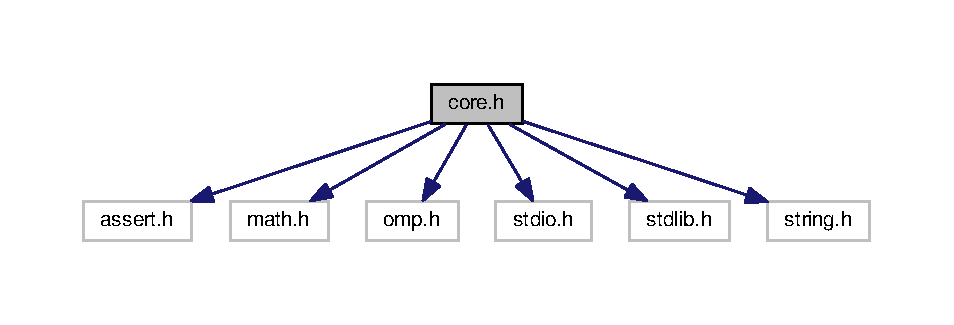
\includegraphics[width=350pt]{core_8h__incl}
\end{center}
\end{figure}
This graph shows which files directly or indirectly include this file\+:
\nopagebreak
\begin{figure}[H]
\begin{center}
\leavevmode
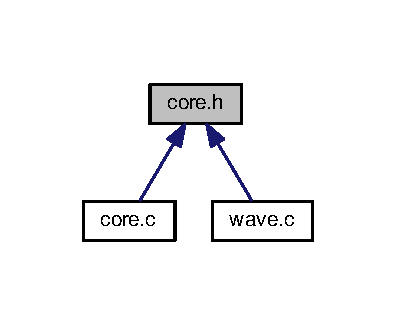
\includegraphics[width=190pt]{core_8h__dep__incl}
\end{center}
\end{figure}
\subsection*{Macros}
\begin{DoxyCompactItemize}
\item 
\#define \hyperlink{core_8h_a85690765490bd5f4d7468932c994d489}{assert\+Equals\+Double}(expected, actual, epsilon)~(assert(fabs((expected) -\/ (actual)) $<$ epsilon));
\end{DoxyCompactItemize}
\subsection*{Functions}
\begin{DoxyCompactItemize}
\item 
void \hyperlink{core_8h_a2c792ddc06951a4c4d72722e4779f144}{init} (double c\+Factor, unsigned int t\+Points, double shift\+Factor)
\item 
void \hyperlink{core_8h_ae251324c29181b9ea249c78be92f5e2f}{simulate} (void)
\item 
void \hyperlink{core_8h_af7c55157c0a3bf716d80e993ae851cf9}{output} (void)
\item 
double $\ast$ \hyperlink{core_8h_a0bcee3285f057c9e07ba0404438fff04}{get\+New\+Values} (void)
\item 
int \hyperlink{core_8h_a38816599a2e623418a5d5b625fbfeeb4}{get\+Array\+Size} (void)
\item 
void \hyperlink{core_8h_a5354b26c0e92bc241bbaf8daedc5a28c}{terminate} (void)
\end{DoxyCompactItemize}


\subsection{Macro Definition Documentation}
\hypertarget{core_8h_a85690765490bd5f4d7468932c994d489}{\index{core.\+h@{core.\+h}!assert\+Equals\+Double@{assert\+Equals\+Double}}
\index{assert\+Equals\+Double@{assert\+Equals\+Double}!core.\+h@{core.\+h}}
\subsubsection[{assert\+Equals\+Double}]{\setlength{\rightskip}{0pt plus 5cm}\#define assert\+Equals\+Double(
\begin{DoxyParamCaption}
\item[{}]{expected, }
\item[{}]{actual, }
\item[{}]{epsilon}
\end{DoxyParamCaption}
)~(assert(fabs((expected) -\/ (actual)) $<$ epsilon));}}\label{core_8h_a85690765490bd5f4d7468932c994d489}


\subsection{Function Documentation}
\hypertarget{core_8h_a38816599a2e623418a5d5b625fbfeeb4}{\index{core.\+h@{core.\+h}!get\+Array\+Size@{get\+Array\+Size}}
\index{get\+Array\+Size@{get\+Array\+Size}!core.\+h@{core.\+h}}
\subsubsection[{get\+Array\+Size}]{\setlength{\rightskip}{0pt plus 5cm}int get\+Array\+Size (
\begin{DoxyParamCaption}
\item[{void}]{}
\end{DoxyParamCaption}
)}}\label{core_8h_a38816599a2e623418a5d5b625fbfeeb4}
Return lengths of the value arrays

\begin{DoxyReturn}{Returns}
lengths 
\end{DoxyReturn}
\hypertarget{core_8h_a0bcee3285f057c9e07ba0404438fff04}{\index{core.\+h@{core.\+h}!get\+New\+Values@{get\+New\+Values}}
\index{get\+New\+Values@{get\+New\+Values}!core.\+h@{core.\+h}}
\subsubsection[{get\+New\+Values}]{\setlength{\rightskip}{0pt plus 5cm}double$\ast$ get\+New\+Values (
\begin{DoxyParamCaption}
\item[{void}]{}
\end{DoxyParamCaption}
)}}\label{core_8h_a0bcee3285f057c9e07ba0404438fff04}
Returns the current state of most recent values.

\begin{DoxyReturn}{Returns}
pointer to array of the newest values 
\end{DoxyReturn}
\hypertarget{core_8h_a2c792ddc06951a4c4d72722e4779f144}{\index{core.\+h@{core.\+h}!init@{init}}
\index{init@{init}!core.\+h@{core.\+h}}
\subsubsection[{init}]{\setlength{\rightskip}{0pt plus 5cm}void init (
\begin{DoxyParamCaption}
\item[{double}]{c\+Factor, }
\item[{unsigned int}]{t\+Points, }
\item[{double}]{shift\+Factor}
\end{DoxyParamCaption}
)}}\label{core_8h_a2c792ddc06951a4c4d72722e4779f144}
Initializes the wave with the results of a sinus function.


\begin{DoxyParams}{Parameters}
{\em c\+Factor} & time step size \\
\hline
{\em t\+Points} & array length \\
\hline
{\em shift\+Factor} & difference between initial waves \\
\hline
\end{DoxyParams}
\hypertarget{core_8h_af7c55157c0a3bf716d80e993ae851cf9}{\index{core.\+h@{core.\+h}!output@{output}}
\index{output@{output}!core.\+h@{core.\+h}}
\subsubsection[{output}]{\setlength{\rightskip}{0pt plus 5cm}void output (
\begin{DoxyParamCaption}
\item[{void}]{}
\end{DoxyParamCaption}
)}}\label{core_8h_af7c55157c0a3bf716d80e993ae851cf9}
Outputs the current state of most recent values. \hypertarget{core_8h_ae251324c29181b9ea249c78be92f5e2f}{\index{core.\+h@{core.\+h}!simulate@{simulate}}
\index{simulate@{simulate}!core.\+h@{core.\+h}}
\subsubsection[{simulate}]{\setlength{\rightskip}{0pt plus 5cm}void simulate (
\begin{DoxyParamCaption}
\item[{void}]{}
\end{DoxyParamCaption}
)}}\label{core_8h_ae251324c29181b9ea249c78be92f5e2f}
Executes on simulation step using the wave equation. \hypertarget{core_8h_a5354b26c0e92bc241bbaf8daedc5a28c}{\index{core.\+h@{core.\+h}!terminate@{terminate}}
\index{terminate@{terminate}!core.\+h@{core.\+h}}
\subsubsection[{terminate}]{\setlength{\rightskip}{0pt plus 5cm}void terminate (
\begin{DoxyParamCaption}
\item[{void}]{}
\end{DoxyParamCaption}
)}}\label{core_8h_a5354b26c0e92bc241bbaf8daedc5a28c}
Frees all allocated memory. 
\hypertarget{wave_8c}{\section{wave.\+c File Reference}
\label{wave_8c}\index{wave.\+c@{wave.\+c}}
}
{\ttfamily \#include $<$gtk/gtk.\+h$>$}\\*
{\ttfamily \#include $<$unistd.\+h$>$}\\*
{\ttfamily \#include $<$pthread.\+h$>$}\\*
{\ttfamily \#include \char`\"{}core.\+h\char`\"{}}\\*
{\ttfamily \#include \char`\"{}config.\+h\char`\"{}}\\*
Include dependency graph for wave.\+c\+:
\nopagebreak
\begin{figure}[H]
\begin{center}
\leavevmode
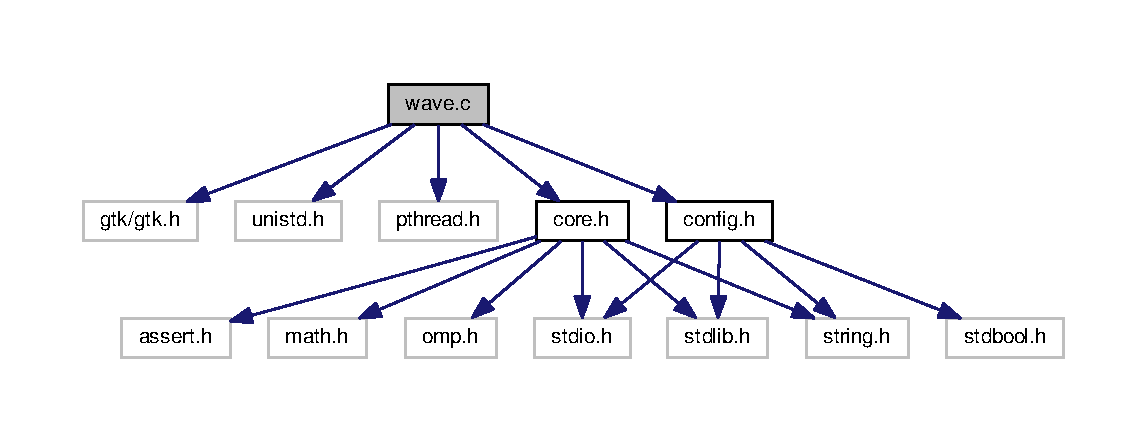
\includegraphics[width=350pt]{wave_8c__incl}
\end{center}
\end{figure}
\subsection*{Macros}
\begin{DoxyCompactItemize}
\item 
\#define \hyperlink{wave_8c_aaf6b22b89bb364988f4882030a309a99}{X\+\_\+\+O\+F\+F\+S\+E\+T}~40
\item 
\#define \hyperlink{wave_8c_aff6396abd8dad0f793f1a4333682a2be}{Y\+\_\+\+O\+F\+F\+S\+E\+T}~20
\item 
\#define \hyperlink{wave_8c_a727ffbbc69f2aeeb24907681dc43a7a6}{M\+A\+G\+N\+I\+F\+I\+C\+A\+T\+I\+O\+N}~50
\item 
\#define \hyperlink{wave_8c_a498d9f026138406895e9a34b504ac6a6}{W\+I\+N\+D\+O\+W\+\_\+\+W\+I\+D\+T\+H}~1200
\item 
\#define \hyperlink{wave_8c_a5473cf64fa979b48335079c99532e243}{W\+I\+N\+D\+O\+W\+\_\+\+H\+E\+I\+G\+H\+T}~315
\end{DoxyCompactItemize}
\subsection*{Functions}
\begin{DoxyCompactItemize}
\item 
gboolean \hyperlink{wave_8c_abf397c7a13188c9084cbfb8fa44a0101}{on\+\_\+window\+\_\+configure\+\_\+event} (Gtk\+Widget $\ast$da, Gdk\+Event\+Configure $\ast$event, gpointer user\+\_\+data)
\item 
gboolean \hyperlink{wave_8c_a160ea893ba694f940cac098f8f748d44}{on\+\_\+window\+\_\+expose\+\_\+event} (Gtk\+Widget $\ast$da, Gdk\+Event\+Expose $\ast$event, gpointer user\+\_\+data)
\item 
void \hyperlink{wave_8c_aa0b970da4405389c144095b04eacd133}{close\+\_\+window} (void)
\item 
void $\ast$ \hyperlink{wave_8c_a139ddc489fa431f04616430c085ee194}{do\+\_\+draw} (void $\ast$ptr)
\item 
gboolean \hyperlink{wave_8c_a4cd40d848edc0f75a94002837921c15a}{timer\+\_\+exe} (Gtk\+Widget $\ast$window)
\item 
int \hyperlink{wave_8c_a0ddf1224851353fc92bfbff6f499fa97}{main} (int argc, char $\ast$argv\mbox{[}$\,$\mbox{]})
\end{DoxyCompactItemize}


\subsection{Macro Definition Documentation}
\hypertarget{wave_8c_a727ffbbc69f2aeeb24907681dc43a7a6}{\index{wave.\+c@{wave.\+c}!M\+A\+G\+N\+I\+F\+I\+C\+A\+T\+I\+O\+N@{M\+A\+G\+N\+I\+F\+I\+C\+A\+T\+I\+O\+N}}
\index{M\+A\+G\+N\+I\+F\+I\+C\+A\+T\+I\+O\+N@{M\+A\+G\+N\+I\+F\+I\+C\+A\+T\+I\+O\+N}!wave.\+c@{wave.\+c}}
\subsubsection[{M\+A\+G\+N\+I\+F\+I\+C\+A\+T\+I\+O\+N}]{\setlength{\rightskip}{0pt plus 5cm}\#define M\+A\+G\+N\+I\+F\+I\+C\+A\+T\+I\+O\+N~50}}\label{wave_8c_a727ffbbc69f2aeeb24907681dc43a7a6}
\hypertarget{wave_8c_a5473cf64fa979b48335079c99532e243}{\index{wave.\+c@{wave.\+c}!W\+I\+N\+D\+O\+W\+\_\+\+H\+E\+I\+G\+H\+T@{W\+I\+N\+D\+O\+W\+\_\+\+H\+E\+I\+G\+H\+T}}
\index{W\+I\+N\+D\+O\+W\+\_\+\+H\+E\+I\+G\+H\+T@{W\+I\+N\+D\+O\+W\+\_\+\+H\+E\+I\+G\+H\+T}!wave.\+c@{wave.\+c}}
\subsubsection[{W\+I\+N\+D\+O\+W\+\_\+\+H\+E\+I\+G\+H\+T}]{\setlength{\rightskip}{0pt plus 5cm}\#define W\+I\+N\+D\+O\+W\+\_\+\+H\+E\+I\+G\+H\+T~315}}\label{wave_8c_a5473cf64fa979b48335079c99532e243}
\hypertarget{wave_8c_a498d9f026138406895e9a34b504ac6a6}{\index{wave.\+c@{wave.\+c}!W\+I\+N\+D\+O\+W\+\_\+\+W\+I\+D\+T\+H@{W\+I\+N\+D\+O\+W\+\_\+\+W\+I\+D\+T\+H}}
\index{W\+I\+N\+D\+O\+W\+\_\+\+W\+I\+D\+T\+H@{W\+I\+N\+D\+O\+W\+\_\+\+W\+I\+D\+T\+H}!wave.\+c@{wave.\+c}}
\subsubsection[{W\+I\+N\+D\+O\+W\+\_\+\+W\+I\+D\+T\+H}]{\setlength{\rightskip}{0pt plus 5cm}\#define W\+I\+N\+D\+O\+W\+\_\+\+W\+I\+D\+T\+H~1200}}\label{wave_8c_a498d9f026138406895e9a34b504ac6a6}
\hypertarget{wave_8c_aaf6b22b89bb364988f4882030a309a99}{\index{wave.\+c@{wave.\+c}!X\+\_\+\+O\+F\+F\+S\+E\+T@{X\+\_\+\+O\+F\+F\+S\+E\+T}}
\index{X\+\_\+\+O\+F\+F\+S\+E\+T@{X\+\_\+\+O\+F\+F\+S\+E\+T}!wave.\+c@{wave.\+c}}
\subsubsection[{X\+\_\+\+O\+F\+F\+S\+E\+T}]{\setlength{\rightskip}{0pt plus 5cm}\#define X\+\_\+\+O\+F\+F\+S\+E\+T~40}}\label{wave_8c_aaf6b22b89bb364988f4882030a309a99}
\hypertarget{wave_8c_aff6396abd8dad0f793f1a4333682a2be}{\index{wave.\+c@{wave.\+c}!Y\+\_\+\+O\+F\+F\+S\+E\+T@{Y\+\_\+\+O\+F\+F\+S\+E\+T}}
\index{Y\+\_\+\+O\+F\+F\+S\+E\+T@{Y\+\_\+\+O\+F\+F\+S\+E\+T}!wave.\+c@{wave.\+c}}
\subsubsection[{Y\+\_\+\+O\+F\+F\+S\+E\+T}]{\setlength{\rightskip}{0pt plus 5cm}\#define Y\+\_\+\+O\+F\+F\+S\+E\+T~20}}\label{wave_8c_aff6396abd8dad0f793f1a4333682a2be}


\subsection{Function Documentation}
\hypertarget{wave_8c_aa0b970da4405389c144095b04eacd133}{\index{wave.\+c@{wave.\+c}!close\+\_\+window@{close\+\_\+window}}
\index{close\+\_\+window@{close\+\_\+window}!wave.\+c@{wave.\+c}}
\subsubsection[{close\+\_\+window}]{\setlength{\rightskip}{0pt plus 5cm}void close\+\_\+window (
\begin{DoxyParamCaption}
\item[{void}]{}
\end{DoxyParamCaption}
)}}\label{wave_8c_aa0b970da4405389c144095b04eacd133}
\hypertarget{wave_8c_a139ddc489fa431f04616430c085ee194}{\index{wave.\+c@{wave.\+c}!do\+\_\+draw@{do\+\_\+draw}}
\index{do\+\_\+draw@{do\+\_\+draw}!wave.\+c@{wave.\+c}}
\subsubsection[{do\+\_\+draw}]{\setlength{\rightskip}{0pt plus 5cm}void $\ast$ do\+\_\+draw (
\begin{DoxyParamCaption}
\item[{void $\ast$}]{ptr}
\end{DoxyParamCaption}
)}}\label{wave_8c_a139ddc489fa431f04616430c085ee194}


Here is the call graph for this function\+:
\nopagebreak
\begin{figure}[H]
\begin{center}
\leavevmode
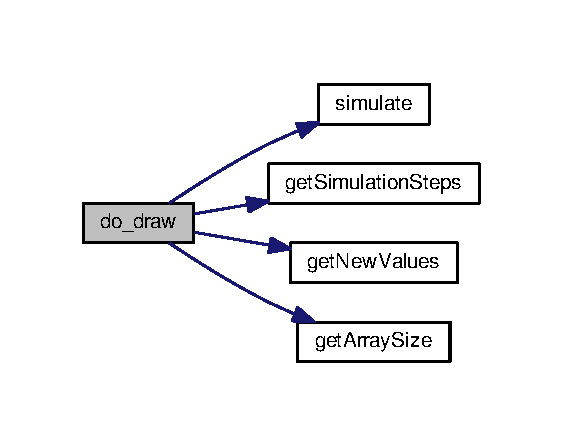
\includegraphics[width=270pt]{wave_8c_a139ddc489fa431f04616430c085ee194_cgraph}
\end{center}
\end{figure}


\hypertarget{wave_8c_a0ddf1224851353fc92bfbff6f499fa97}{\index{wave.\+c@{wave.\+c}!main@{main}}
\index{main@{main}!wave.\+c@{wave.\+c}}
\subsubsection[{main}]{\setlength{\rightskip}{0pt plus 5cm}int main (
\begin{DoxyParamCaption}
\item[{int}]{argc, }
\item[{char $\ast$}]{argv\mbox{[}$\,$\mbox{]}}
\end{DoxyParamCaption}
)}}\label{wave_8c_a0ddf1224851353fc92bfbff6f499fa97}


Here is the call graph for this function\+:
\nopagebreak
\begin{figure}[H]
\begin{center}
\leavevmode
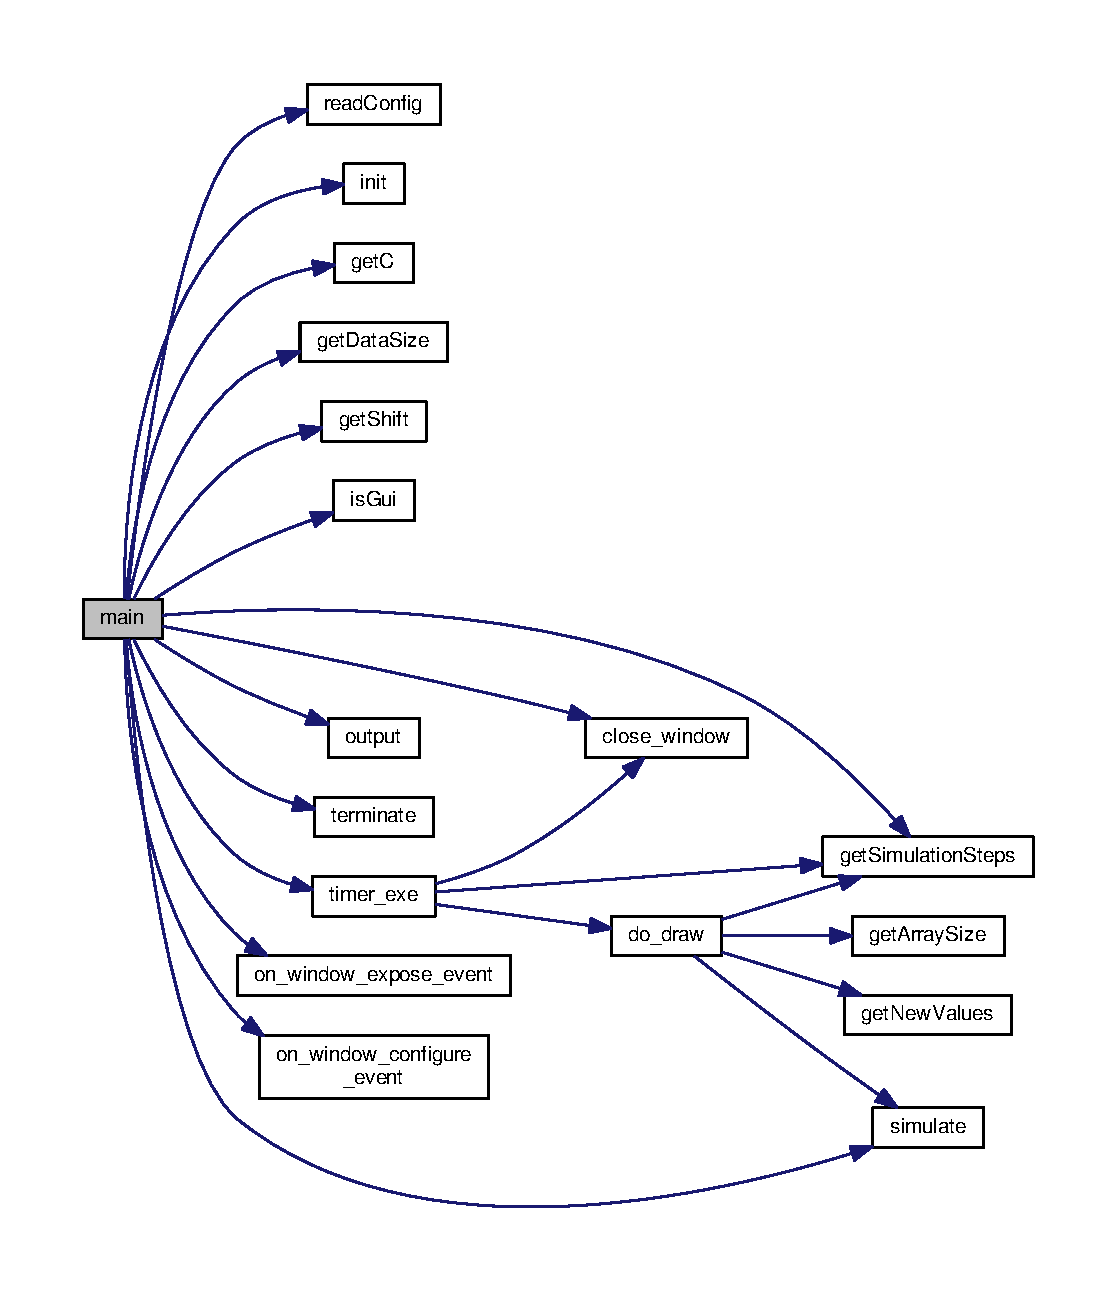
\includegraphics[width=350pt]{wave_8c_a0ddf1224851353fc92bfbff6f499fa97_cgraph}
\end{center}
\end{figure}


\hypertarget{wave_8c_abf397c7a13188c9084cbfb8fa44a0101}{\index{wave.\+c@{wave.\+c}!on\+\_\+window\+\_\+configure\+\_\+event@{on\+\_\+window\+\_\+configure\+\_\+event}}
\index{on\+\_\+window\+\_\+configure\+\_\+event@{on\+\_\+window\+\_\+configure\+\_\+event}!wave.\+c@{wave.\+c}}
\subsubsection[{on\+\_\+window\+\_\+configure\+\_\+event}]{\setlength{\rightskip}{0pt plus 5cm}gboolean on\+\_\+window\+\_\+configure\+\_\+event (
\begin{DoxyParamCaption}
\item[{Gtk\+Widget $\ast$}]{da, }
\item[{Gdk\+Event\+Configure $\ast$}]{event, }
\item[{gpointer}]{user\+\_\+data}
\end{DoxyParamCaption}
)}}\label{wave_8c_abf397c7a13188c9084cbfb8fa44a0101}
\hypertarget{wave_8c_a160ea893ba694f940cac098f8f748d44}{\index{wave.\+c@{wave.\+c}!on\+\_\+window\+\_\+expose\+\_\+event@{on\+\_\+window\+\_\+expose\+\_\+event}}
\index{on\+\_\+window\+\_\+expose\+\_\+event@{on\+\_\+window\+\_\+expose\+\_\+event}!wave.\+c@{wave.\+c}}
\subsubsection[{on\+\_\+window\+\_\+expose\+\_\+event}]{\setlength{\rightskip}{0pt plus 5cm}gboolean on\+\_\+window\+\_\+expose\+\_\+event (
\begin{DoxyParamCaption}
\item[{Gtk\+Widget $\ast$}]{da, }
\item[{Gdk\+Event\+Expose $\ast$}]{event, }
\item[{gpointer}]{user\+\_\+data}
\end{DoxyParamCaption}
)}}\label{wave_8c_a160ea893ba694f940cac098f8f748d44}
\hypertarget{wave_8c_a4cd40d848edc0f75a94002837921c15a}{\index{wave.\+c@{wave.\+c}!timer\+\_\+exe@{timer\+\_\+exe}}
\index{timer\+\_\+exe@{timer\+\_\+exe}!wave.\+c@{wave.\+c}}
\subsubsection[{timer\+\_\+exe}]{\setlength{\rightskip}{0pt plus 5cm}gboolean timer\+\_\+exe (
\begin{DoxyParamCaption}
\item[{Gtk\+Widget $\ast$}]{window}
\end{DoxyParamCaption}
)}}\label{wave_8c_a4cd40d848edc0f75a94002837921c15a}


Here is the call graph for this function\+:
\nopagebreak
\begin{figure}[H]
\begin{center}
\leavevmode
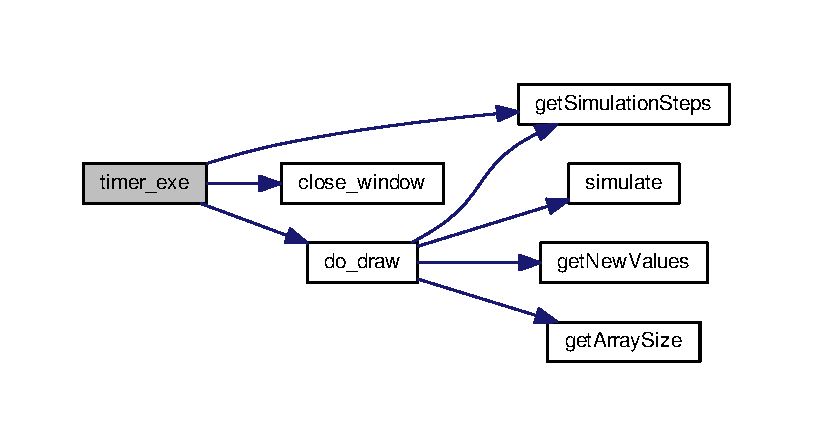
\includegraphics[width=350pt]{wave_8c_a4cd40d848edc0f75a94002837921c15a_cgraph}
\end{center}
\end{figure}



%--- End generated contents ---

% Index
\newpage
\phantomsection
\addcontentsline{toc}{chapter}{Index}
\printindex

\end{document}
